% !TeX spellcheck = en_AU-EnglishAustralia
% Preamble
\documentclass[9pt, a4paper]{report}
\usepackage[utf8]{inputenc}
\usepackage{indentfirst}
\usepackage{rotating, graphicx}
\usepackage{geometry}

\newgeometry{vmargin={30mm}}

\title{E14 Wellnomics Project Proposal}
\author{Laurence Prins, Toby Bourke,  Aryan Srivastava,  Bill Liu}
\date{21.03.2021}

\widowpenalties 1 10000
\raggedbottom

\begin{document}
	\begin{center}
		\section*{\Huge Final Year Project Proposal E14}
	\end{center}
	
	\vspace{60pt} \hfill \pagenumbering{gobble}
	
	\noindent\textbf{Project Title:} Indoor Positioning and Asset Tracking\\
	
	\noindent\textbf{Supervisor:} Shayne Crimp, Diego Ramirez\\
	
	\noindent\textbf{Industrial Sponsor:} Kevin Taylor\\
	
	\noindent\textbf{Student Names:} Laurence Prins, Bill Liu, Toby Bourke, Aryan Srivastava\\
	
	\noindent\textbf{Student ID Numbers:} 84063049, 49791816, 84984154, 43958596\\
	
	\noindent\textbf{Student Emails:} ltp17@uclive.ac.nz, pli49@uclive.ac.nz, tfb20@uclive.ac.nz, asr62@uclive.ac.nz\\
	
	\pagebreak
	
	\maketitle
	
	\pagenumbering{arabic}
	\section*{Purpose Statement}
	The purpose of this project is to develop software for a device that improves the well-being of
employees and the ergonomics of office spaces. The project will deliver an indoor mapping system
through the use of audio technology.
	% -------------------------------------- BACKGROUND AND SCOP ---------------------
	\section*{Background and Scope}
	\subsection*{Background}
	
	Wellnomics is a company that develops systems to improve the health, well-being and productivity of computer users. The systems designed primarily are software solutions to improve the ergonomics of various systems. Software Wellnomics has produced include but is not limited to ``Micro-pause \&
stretch break coaching'' and ``Human factors and ergonomics Management Reporting''.\\

	The software that Wellnomics produces benefit employees and managers alike. Wellnomics’s ``Micropause...'' software can decrease the risk of employees getting Occupational Overuse Syndrome (OOS). OOS occurs when the same action is done many times repeatedly, and the software prompts the user periodically to take a break and stretch. The ``Human factors...'' software Wellnomics produces can be used by managers to track how at-risk specific employees are.\\

	To improve the well-being of employees, Wellnomics is developing a device that can track a significant amount of information on how an employee is working. Information being tracked includes but is not limited to temperature, desk height, and whether the employee is typing. To further expand the capabilities of the device, Wellnomics wants to create a 3D mesh of all the devices. This 3D mesh will provide information on where the devices are within an environment. Wellnomics requires the finding distances between the devices using a currently on-board MEMs microphone and speaker.

	\subsection*{Justification}
	
	Wellnomics requires a 3D mesh of the devices to accurately model how space is laid out or where specific objects are located. The goal of this 3D mesh is to increase the ergonomics of an environment significantly. This ergonomic improvement can come in many different forms. An example of an environment that the 3D mesh that can be implemented is an office with hot-desks.\\

	Using the 3D mesh within a hot-desk office would allow for accurate tracking of how location can affect the employees. The 3D mesh would be able to give insight into how the office space is being used. Using data from the devices and various pieces of software Wellnomics has produced would allow managers a comprehensive picture of how their employees perform. Managers would be able to improve the environment to encourage healthier behaviours and increased performance in employees.
	
	\subsection*{Description (User requirements and specification)}
	Audio waves travel at a specific speed through a given medium. For example, in dry air at 20$^{\circ}$ C, the speed of sound is 343 m/s. If the time of travel between two points is known, then the distance between these two points can be calculated. If two devices are synced up, then by sending a pulse, and timing the response, an accurate measurement of distance can be produced.\\
	
	A grid of devices will be able to produce distance measurements between each other to create a map. The goal is to get these measurements within 90\% accuracy and send this data back to a central system that requested the scan. The team will produce software whereby a user can request a map of the locations of all the surrounding devices. The devices will then ping each other to generate distance measurements and return this data back to the user. By using the data, an accurate map of the current positions of each device will be generated. \\
	
	\subsection*{Deliverables and Outcomes}
	Initial research will be focused on the significant technologies involved in the project. Namely, these are the sound devices (microphone and speaker), the mesh communications network, the indoor mapping and the actual sound used to measure distance. Researching this will enable the team to understand better the specific technologies involved in the development of the device.\\
	
	Once the research is done, a test board can be made to test the findings. This will include testing the range of the microphone and speaker, the effects of attenuation and finding the best waveform for the application. Various environmental factors can affect sound waves, such as temperature and humidity. These need to be examined along with the attenuation of sound due to obstructions. Testing will help the team uncover the limits of technology in different scenarios.\\
	
	Throughout the year, to ensure the team is on track, there will be a progress report and an oral progress inspection. The final project will be delivered in the form of three deliverables:
	\begin{itemize}
		\item A poster 
		\item A presentation 
		\item The completed software 
	\end{itemize}
	These will be completed within two weeks of the due date to ensure the tasks are done to a satisfactory level.
	\subsection*{Constraints}
	Wellnomics wanted to generate the first prototype as cheap as possible. Some constraints have been created with the hardware limitation and the strategies to solve some of the problems. These prototypes contain a 5V speaker and a digital MEMs microphone. Acoustic distance measurement is used to measure the distance between prototypes within the 3D distance mesh. To provide a more accurate testing result, an anechoic chamber needs to be used to reduce the ambient noise and airflow of testing.\\
	
	% --------------------------------- ADMIN ------------------------------------------
	\section*{Administration}
		
		\subsection*{Group organisation}
			The group contains two mechatronic engineering students, one electrical engineering student and one computer engineering student. The project has been split into four parts. Each group member takes responsibility for one part.
		\subsection*{Group culture}
			Two or more meetings weekly are required to generate a good result and improve communication. Within the group, group members should ask for help when they are falling behind and struggling. Group members should help other group members when they can help without falling behind. Group members should not blame each other for mistakes but encourage each other to generate better work.
		\subsection*{Communication }
			Good communication in group projects is more important than personal knowledge, competence or past performances. Messenger is used between group members to communicate ideas and meeting times. Email communication is used between group members and technician, group members and supervisor, and group members and sponsor.\\
			
	Available group meeting times are collected from everybody using Doodle Poll. Group meetings are arranged by email with calendar invites to remind all attendees of when and where the meeting is taking place and the meeting agenda to describe how the meeting will run. Group meetings are split into three types by the attendees. The meeting types are group members, group members joined with technician and supervisor, and group members joined with technician, supervisor and sponsor. \\
	
	Group meetings with only group members are set for every Friday from 10:00 am onwards. The purpose of this meeting is to generate design ideas, background research of design ideas, problem-solving for chosen design ideas, and implement tests to the design ideas. \\
			
			Group meetings of group members joined with the technician and the supervisor is arranged when needed. The purpose of this meeting is to help with design ideas and further improvements in design ideas, design decisions, and test results.\\
			
			A group meeting of group members, technician, supervisor and sponsor is set every Tuesday from 12:00 pm to 1:00 pm. The purpose of this meeting is to discuss project requirements, report project progress, and finalise design decisions.
		\subsection*{Decision making}
			Each group member takes responsibility for one aspect of the work. Group member makes the decision during the Friday group meetings. All group members collaborate to make design decisions. The group member who has done the most research has the most authority in making the decision. Other group members ask questions about the decision or help to make the decision better.  
		\subsection*{Note-taking}
			During each meeting, one group member should take meeting notes. Meeting notes includes the date, location, start time, finish time, attendees, and essential notes. Meeting notes is used to help group members to review what has been discussed during the meeting.  
		\subsection*{Leadership}
			The group structure is hierarchical. During group formation,  some group members are more outgoing than other group members, and they naturally take leadership roles. To improve other group members’ skills to lead, each group member takes the leadership role for two weeks. The group leader takes the responsibility of organising group meetings, booking meeting rooms and assigns one group member to record meeting notes.
		\subsection*{Central docs}
			All documentations generate from meetings, researches, tests, and programming are stored in a University of Canterbury GitLab cloud space.  All group members can assess and modify the documents. 
	
	% ---------------------- TIMELINE ------------------------------------------
	\section*{Timeline}
	
	\subsection*{Specific Tasks}
	The specific task and the timeline of these tasks are expressed in Appendix A, a Gantt Chart. This chart illustrates the split of subtasks and the potential time required to complete them. With the times, it is important to remember that this is not the sole focus of the group members. The expected contact time for the project is only nine hours per week per student, and as such, some tasks have larger timelines, as they are not the singular focus of the week.\\
	
%	\begin{figure}[!htb]
%		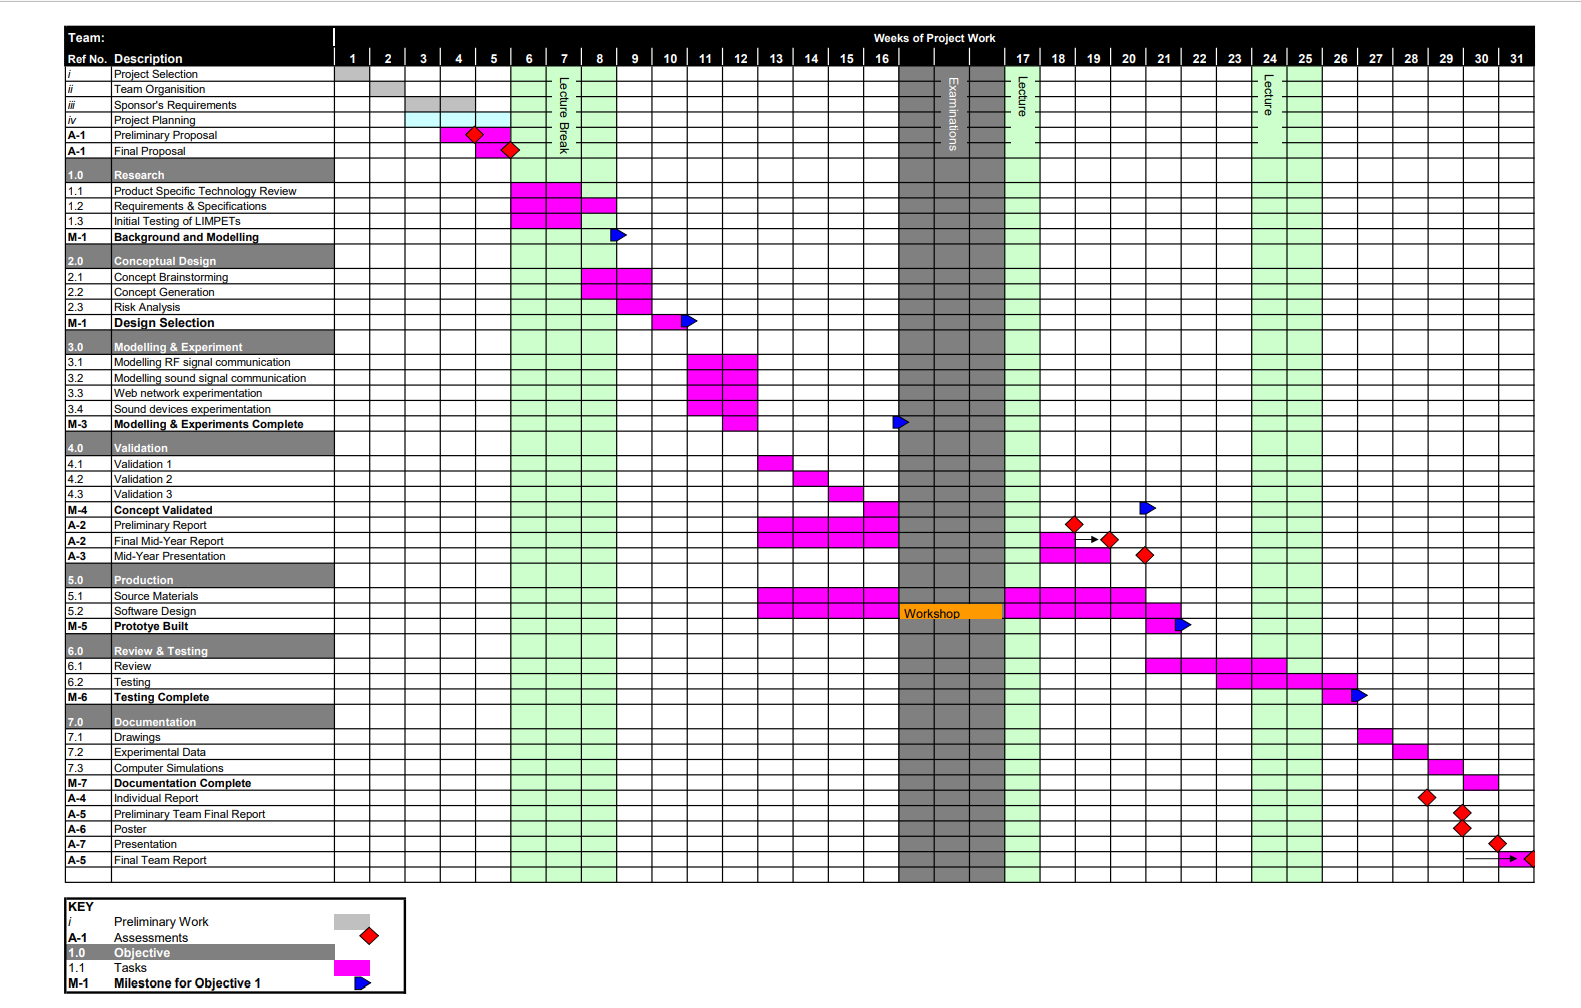
\includegraphics[width=\textwidth]{./Figures/Gnatt}
%		\caption{Gantt Chart for FYP E14}
%		\label{fig:Gantt}
%	\end{figure}
	
	% ------------------------------------ BUDGET ------------------------------
	\section*{Budget}
	\noindent
	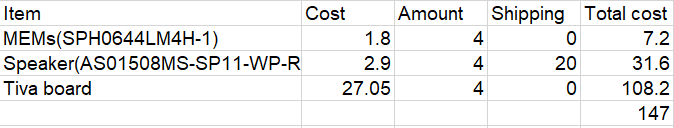
\includegraphics[width=\textwidth]{./Figures/Budget}
	
	\pagebreak

	
	\section*{Appendix A}
		\noindent
		\begin{minipage}{\textwidth}
	    \centering
		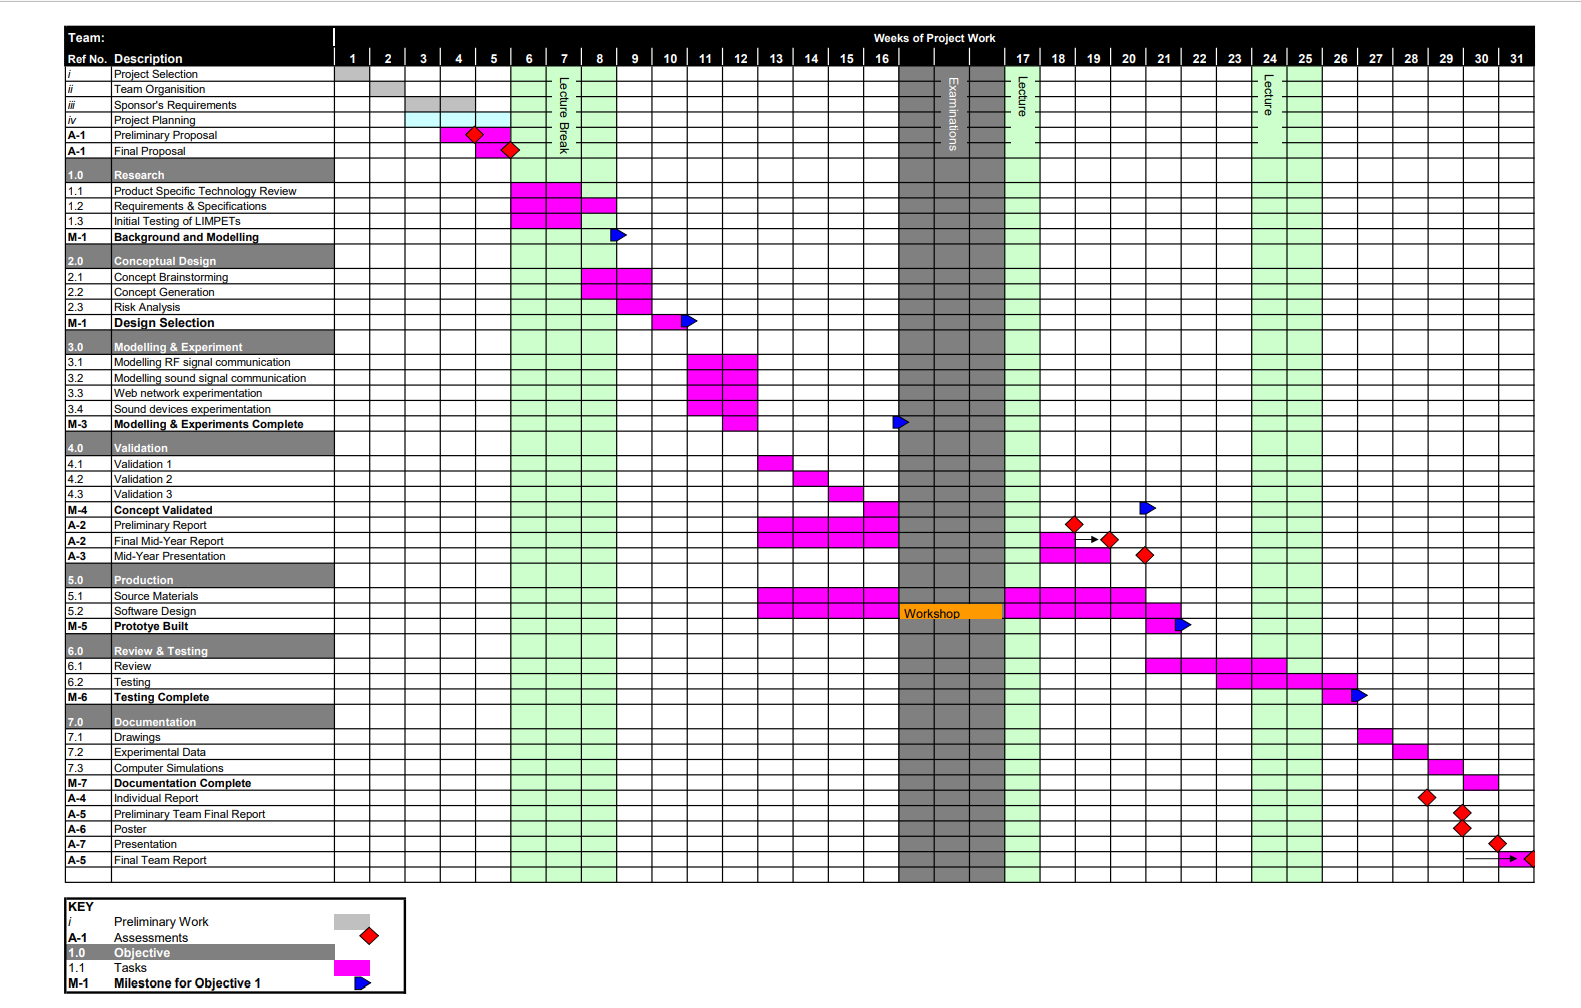
\includegraphics[angle = 90, width=\hsize]{./Figures/Gnatt}
	\end{minipage}
\end{document}
